\section*{Assignment 05: Governance and Data Policies}
\addcontentsline{toc}{section}{Assignment 05: Governance and Data Policies}

\subsection*{Onboarding, feedback loops, and moderation}
Onboarding mixes story with friction tests. Students and NGOs start on separate landing tracks, then move through three phases: pre-signup nudges, profile setup with suggested answers, and a ``first mission'' checklist that unlocks badges once the core features are touched. Mentors or automated prompts reply within the first hour so nobody stalls alone.

Feedback rides inside the workflow. Every core action triggers a one-click rating and optional note, adoption is monitored through cohort dashboards, and weekly summaries go to both sides so the recent wins stay visible \citep{Reillier2017}. Moderation runs across automated filters, trusted community reviewers, and a professional team that handles escalations within a day even if we occasionally pause a thread to gather context.

\subsection*{Data policies and ethics}
We collect only what fuels matching and trust: profile basics, project history, and quality feedback. Data use follows a strict order—service improvement, fair personalisation, and finally aggregated insights for partners—so we avoid the overreach \citet{Zuboff2019} warns about. Differential privacy protects reports, while manual export audits and fairness checks catch the edge cases \citep{Srnicek2017}.

Transparency is built in. A ``data mirror'' page lists every stored datapoint with its purpose, retention timeline, and an edit or delete button. Quarterly accountability notes recap moderation stats, security incidents, and algorithm updates, and an internal ethics board forces product teams to justify experiments before they ship \citep{Choudary2016}.

Figure~\ref{fig:onboarding-flow} shows the guided tour that keeps time-to-first-value under fifteen minutes. Students work through tasks like ``complete portfolio'' and ``book intro call'' while NGOs publish their first brief and assign an owner, aided by short Loom explainers.

\begin{figure}[h]
  \centering
  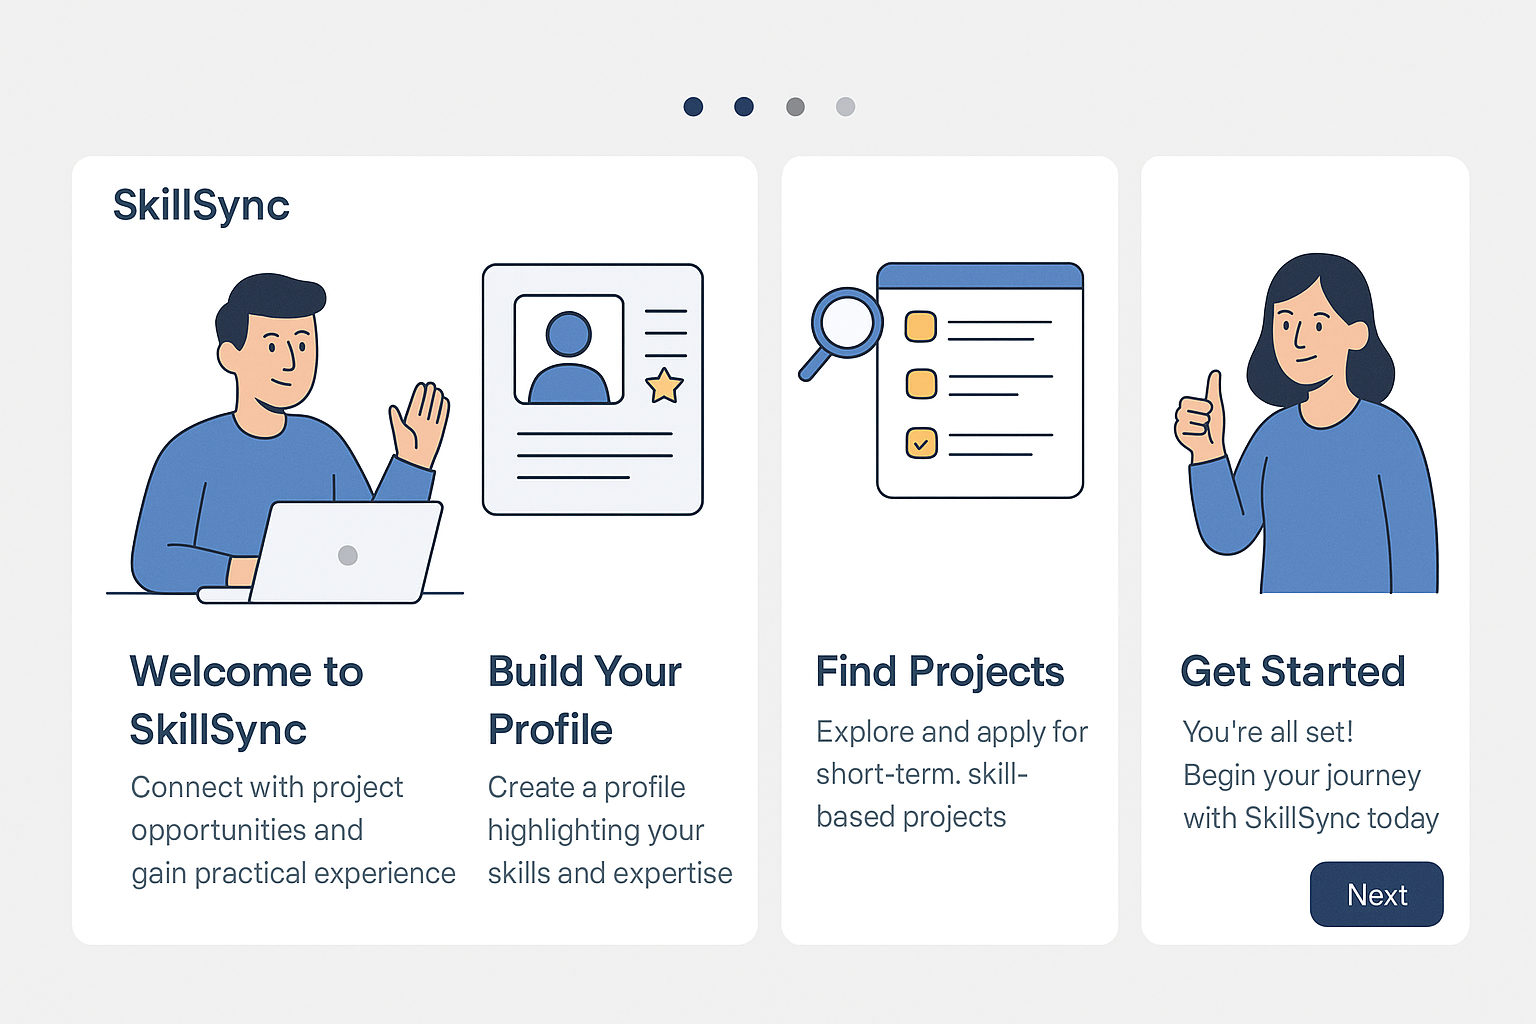
\includegraphics[width=0.85\linewidth]{figures/opgave05/onboarding-flow-ny-bruger.png}
  \caption{Guided onboarding flow (`onboarding-flow-ny-bruger.png`) that compresses time-to-first-value for both sides.}
  \label{fig:onboarding-flow}
\end{figure}

Governance work continues in the admin dashboard (Figure~\ref{fig:admin-panel}). Moderators track flags, disputes, and algorithm signals in one place, with fairness metrics surfaced next to operational stats. They can send templated responses, escalate tricky cases, or log manual follow-ups when automation misreads sarcasm. The audit trail from those actions feeds the accountability notes above.

\begin{figure}[h]
  \centering
  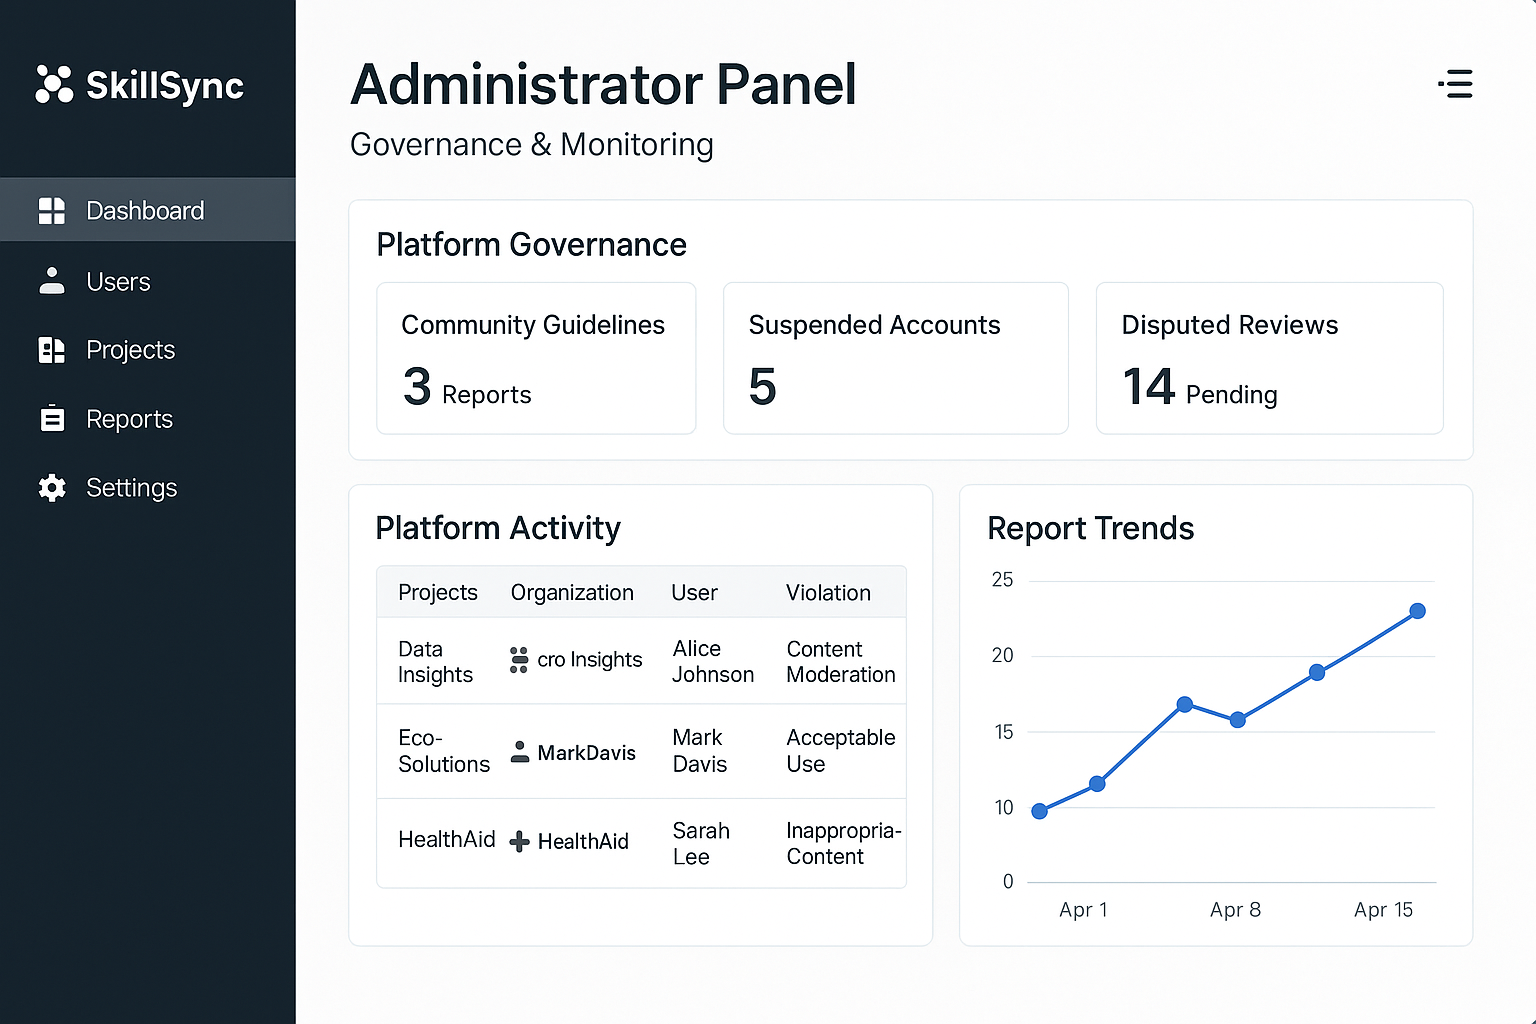
\includegraphics[width=0.85\linewidth]{figures/opgave05/administratorpanel-governance.png}
  \caption{Governance control room (`administratorpanel-governance.png`) used by moderators and the ethics council.}
  \label{fig:admin-panel}
\end{figure}

Communication rituals keep the system humane. We script product nudges in the same voice as onboarding, train moderators in trauma-informed responses, and host quarterly town halls where power users challenge the rules. When early adopters called the policies heavy-handed we added an open moderation retro and publish the resulting action list so changes stay transparent.
